\chapter{System do prowadzenia projektów}

Rozdział ten opisuje autorski system do prowadzenia projektów w trzech wersjach, każda z~nich różni się zastosowanym modelem i bazą danych.
Powstały dwie wersje odpowiednio dla baz Apache Cassandra i MongoDB, oraz trzeci wariant z modelem hybrydowym, gdzie część danych jest przechowywana w bazie relacyjnej, a część w bazie nierelacyjnej.
Główna część systemu powstała jako rezultat pracy inżynierskiej.
Niniejsza praca bazuje na nim rozszerzając nieznacznie jego funkcjonalność w celu dogłębniejszej analizy możliwości porównywanych baz.

% \section{Specyfikacja wymagań funkcjonalnych}

% Jedną z najważniejszych faz rozwoju oprogramowania jest wyspecyfikowanie wymagań.
% Jest to część inżynierii oprogramowania dostarczająca nam środków i metod umożliwiających zebranie na temat funkcjonalności tworzonej przez nas aplikacji lub systemu komputerowego.
% Popełnienie błędu w tej fazie projektu jest najbardziej kosztowne, ponieważ jest to początkowa faza i błędy w niej popełnione propagują się na kolejne fazy.

% \subsection*{Role i uprawniania użytkowników w systemie}

% W opisywanym systemie do prowadzenie projektów można wyróżnić następujące role i powiązane z nimi uprawnienia:
% \begin{itemize}
%     \item \textbf{Użytkownikiem} jest każdy, kto posiada zarejestrowane konto w aplikacji.
%     \item \textbf{Administratorem projektu} staje się użytkownik aplikacji w momencie, gdy stworzy nowy projekt.
%     Daje mu to uprawnienia do:
%     \begin{itemize}
%         \item dodawania nowych zadań w projekcie,
%         \item usuwania istniejących zadań,
%         \item usunięcia administrowanego projektu.
%     \end{itemize}
%     \item \textbf{Uczestnikiem zadania} staje się użytkownik, który został przypisany do zadania przez administratora.
%     Dzięki temu zyskuje uprawnienia do:
%     \begin{itemize}
%         \item dodawania nowego pliku do zadania,
%         \item pobrania wybranej wersji pliku,
%         \item zaznaczenia pliku do zatwierdzenia przez administratora zadania,
%         \item zapisania nowej wersji pliku,
%         \item wyświetlenia szczegółowych informacji o wersji pliku.
%     \end{itemize}
%     \item \textbf{Administratorem zadania} zostaje użytkownik aplikacji, który został wybrany do tego przez administrator projektu podczas tworzenia zadania.
%     Otrzymuje on wtedy następujące przywileje:
%     \begin{itemize}
%         \item możliwość przypisania/usunięcia uczestnika do/z administrowanego zadania,
%         \item możliwość zatwierdzenia ostatecznej wersji pliku,
%         \item możliwość usunięcia pliku.
%     \end{itemize}
%     Oprócz tych uprawnień użytkownik pełniący tą rolę otrzymuje wszystkie uprawniania uczestnika projektu.
% \end{itemize}

% Jeden użytkownik może pełnić wiele z wyżej wymienionych ról.
% Pełniąc je dziedziczy wymienione uprawnienia. 

% \subsection*{Przypadki użycia}

% Przypadki użycia opisywanego systemu zostały podzielone na dwie grupy funkcjonalne.
% Ma to na celu łatwiejsze zrozumienie oferowanej przez system funkcjonalności.

% \subsubsection{Funkcjonalność związana z projektami i zadaniami}

% Zbiór przypadków użycia związany z zarządzaniem projektami i zadaniami w systemie:
% \begin{enumerate}
%     \item \textbf{Utworzenie projektu} -- każdy użytkownik systemu może utworzyć i zarządzać swoimi projektami.
%     \item \textbf{Wyświetlenie listy projektów}, w których uczestniczy użytkownik jest wyświetlane tuż po zalogowaniu się do aplikacji.
%     \item \textbf{Wyświetlenie szczegółowych informacji o projekcie wraz z listą zadań} -- użytkownik może wyświetlić informacje o projekcie jeżeli jest uczestnikiem projektu tzn. jest administratorem projektu, lub administratorem lub uczestnikiem zadania.
%     \item \textbf{Wyświetlenie szczegółowych informacji o zadaniu wraz z listą plików} -- użytkownik może wyświetlić informacje o zadaniu jeżeli jest przypisany do niego, lub jest jego administratorem.
%     \item \textbf{Dodanie nowego zadania do projektu} -- uprawniony do tego jest administrator projektu.
%     \item \textbf{Usunięcie zadania} -- uprawniony do tego jest administrator projektu.
%     \item \textbf{Usunięcie projektu} -- uprawniony do tego jest administrator projektu.
%     \item \textbf{Przypisanie nowego uczestnika do zadania} -- ta funkcja jest dostępna dla administratora zadania.
%     \item \textbf{Usunięcie uczestnika z zadania} -- ta funkcja jest dostępna dla administratora zadania.
% \end{enumerate}

% \subsubsection{Funkcjonalność związana z plikami i ich wersjami}

% Przypadki użycia związane z wszystkimi czynnościami, które można wykonać w~związku z~plikami w~obrębie systemu:
% \begin{enumerate}
%     \item \textbf{Wyszukiwanie pełnotekstowe wśród plików zadania/projektu} jest rozszerzeniem funkcjonalności systemu w porównaniu do systemu powstałego w pracy inżynierskiej.
%     Ten przypadek użycia ma na celu zbadanie możliwości i wsparcia wyszukiwania pełnotekstowego przez bazy danych.
%     Wyszukiwanie to jest dostępne dla uczestników projektów i zadań.
%     Można je uruchomić z poziomu widoku listy zadań -- wtedy zostaną przeszukane wszystkie pliki zadań, do których użytkownik ma dostęp.
%     Wyszukiwanie z widoku listy plików w zadaniu ogranicza przeszukiwane pliki do tych, które znajdują się w zadaniu.
%     Po wyświetleniu listy plików dopasowanych do wyszukiwanej frazy można wybrać jeden z nich i przejść do szczegółowych informacji o nim.
%     \item \textbf{Zatwierdzenie pliku} -- przypadek użycia przeznaczony dla administratora zadania. 
%     Może być zrealizowany gdy system wyświetla listę plików przypisanych do zadania. 
%     Po wybraniu pozycji z tej listy administrator wybiera opcję zatwierdzenia. 
%     Po tej czynności plik posiada status zatwierdzony i nie może można go już edytować.
%     \item  \textbf{Usunąć plik} może tylko administrator zadania. 
%     Wraz z plikiem usuwane są wszystkie zapisane wersje. 
%     W celu usunięcia pliku administrator wybiera pozycję z listy plików i~wybiera opcję usunięcia.
%     \item \textbf{Wyświetlenie szczegółów pliku z listą wersji} -- uprawniony do tego jest uczestnik zadania.
%     Może tego dokonać w poziomu widoku listy plików.
%     \item \textbf{Dodanie nowego pliku} -- funkcjonalność dostępna dla każdego uczestnika zadania. 
%     \item \textbf{Pobranie wersji pliku} -- dostępne dla uczestnika zadania. 
%     Po przejściu do widoku listy wersji pliku może wybrać opcję pobrania konkretnej wersji.
%     \item \textbf{Zaznaczenie pliku do zatwierdzenia przez administratora zadania} -- prosty przypadek użycia dostępny dla uczestnika zadania.
%     Po wyświetleniu  szczegółowego widoku informacji o pliku może wybrać opcję oznaczenia pliku do zatwierdzania.
%     \item \textbf{Zapisanie nowej wersji pliku} jest dostępne dla uczestnika zadania z poziomu widoku szczegółowych informacji o pliku.
%     \item \textbf{Wyświetlenie szczegółowych informacji o wersji pliku} -- opcja dostępna dla uczestników zadania.
% \end{enumerate}

\section{Funkcjonalność systemu}

Główną funkcjonalnością systemu jest tworzenie projektów oraz zarządzanie nimi poprzez dodawanie lub usuwanie zadań.
Rysunek~\ref{fig:sysFunProject} przedstawia widok z informacjami o szczegółach projektu, do którego ma dostęp zalogowany użytkownik.
Widzi również na nim listę zadań w~projekcie, w których bierze udział.
Dodatkowo administrator projektu może z poziomu tego widoku dodawać zadania lub usunąć całkowicie projekt.

\begin{figure}[!ht]
\centering
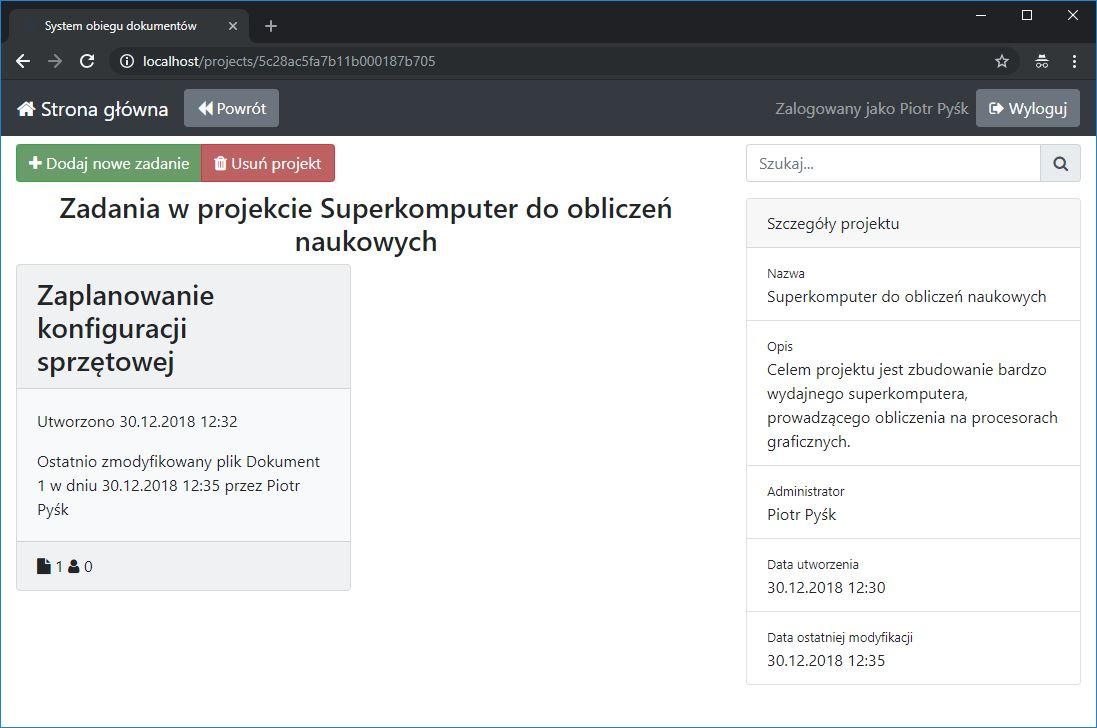
\includegraphics[width=0.8\textwidth]{figures/projekt.JPG}
\caption{Widok szczegółowych informacji o projekcie}
\label{fig:sysFunProject}
\end{figure}

Po przejściu do zadania ukazuje się użytkownikowi widok przedstawiony na Rysunku~\ref{fig:sysFunTask}.
Z poziomu tego widoku może przejść do szczegółowych informacji o wybranym pliku w zadaniu.
Administrator projektu może przejść do zakładki panelu administracyjnego zadania, który pozwala mu na usunięcie zadania wraz z przypisanymi do niego dokumentami.

\begin{figure}[!ht]
\centering
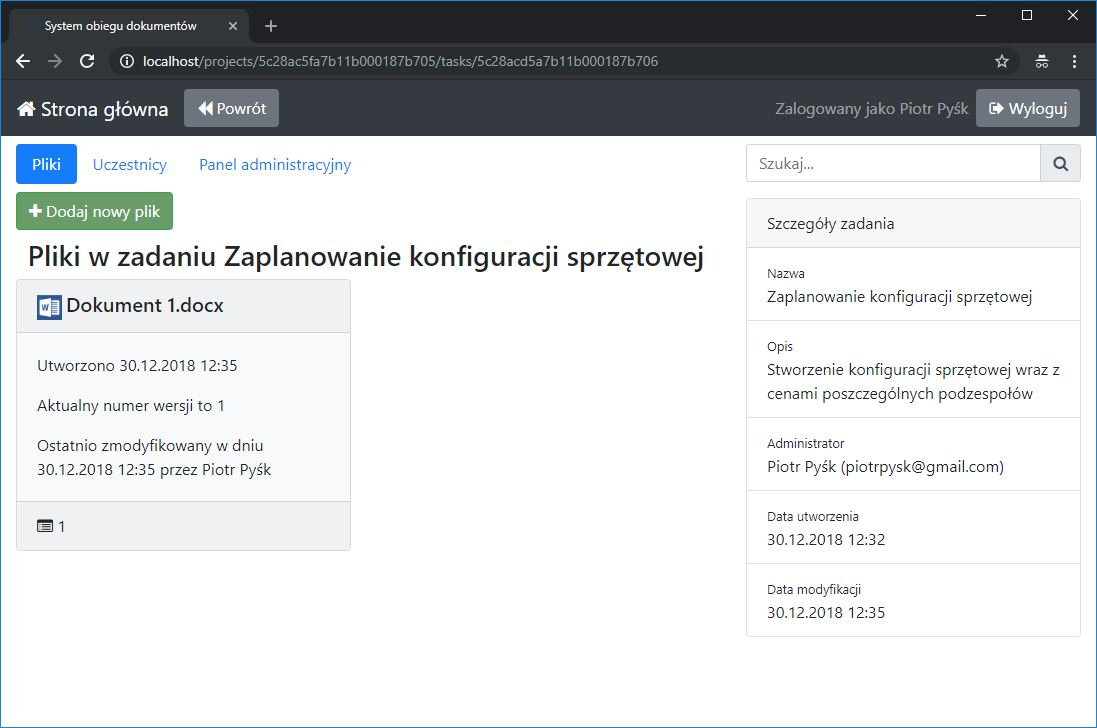
\includegraphics[width=0.8\textwidth]{figures/Zadanie.JPG}
\caption{Widok szczegółowych informacji o zadaniu}
\label{fig:sysFunTask}
\end{figure}

Kolejną z funkcji jakie dostarcza system jest proste wersjonowanie dokumentów przechowywanych w zadaniach.
Służy to np. do zobrazowania postępu w tworzeniu ważnego dokumentu, lub szybkiego sprawdzenia zmian dokonanych przez innych użytkowników.
W ramach rozszerzenia funkcjonalności systemu powstało wyszukiwanie pełnotekstowe plików.
Funkcjonalność ta została stworzona w ramach niniejszej pracy w celu zbadania możliwości wyszukiwania pełnotekstowego oferowanego przez porównywane bazy nierelacyjne.

Z poziomu przedstawionych wcześniej widoków szczegółowych informacji o projekcie i zadaniu możliwe jest wyszukiwanie plików zawierających zadaną frazę.
Wystarczy wpisać ją w pole znajdujące się w prawym górnym rogu i nacisnąć klawisz \textit{Enter}.
Następnie aplikacja wyświetla listę dopasowanych dokumentów, wraz z ich nazwami, oraz nazwami zadań, do których są przypisane.
Rysunek~\ref{fig:sysFunSearch} przedstawia przykładowy widok wyników wyszukiwania.

\begin{figure}[!ht]
\centering
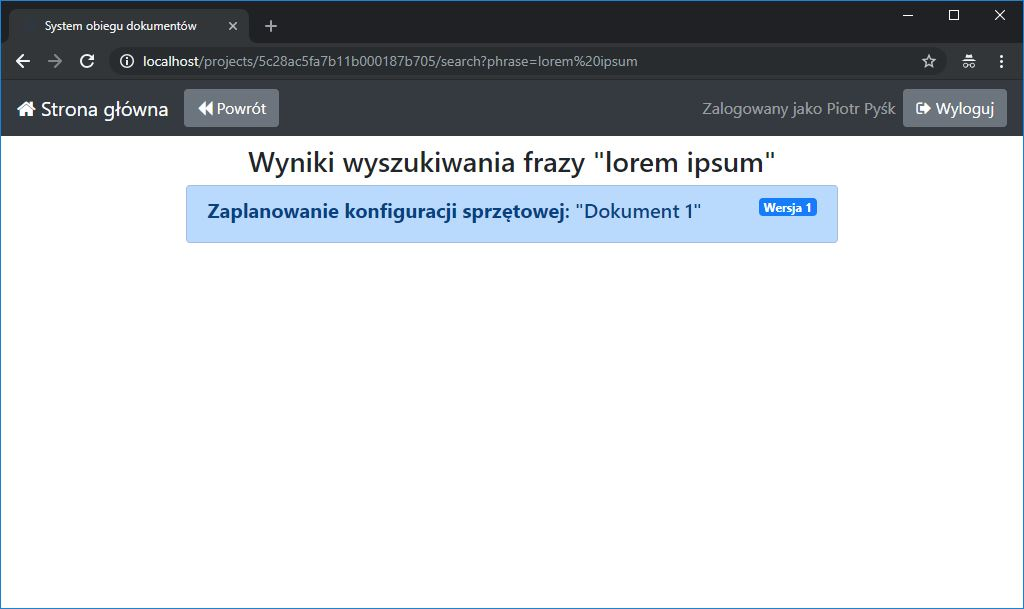
\includegraphics[width=0.8\textwidth]{figures/wyniki_wyszukiwania.JPG}
\caption{Widok wyników wyszukiwania zadanej frazy}
\label{fig:sysFunSearch}
\end{figure}

Z listy plików w zadaniu i wyników wyszukiwania możliwe jest przejście do szczegółowych informacji o pliku.
Rysunek~\ref{fig:sysFunFile} przedstawia przykładowy widok informacji o pliku.
Znajduje się na nim lista jego wersji posortowana w odwrotnej kolejności chronologicznej.
Każdą z tych wersji można pobrać lub wyświetlić jej zawartość tekstową.
Uczestnik zadania może również dodać kolejną wersję pliku.
Administrator zadania może zatwierdzić plik, dzięki czemu nie będzie już możliwe dodanie jego nowej wersji.
Jest też możliwość usunięcia pliku przez administratora zadania, wraz z jego całą historią wersji.

\begin{figure}[!ht]
\centering
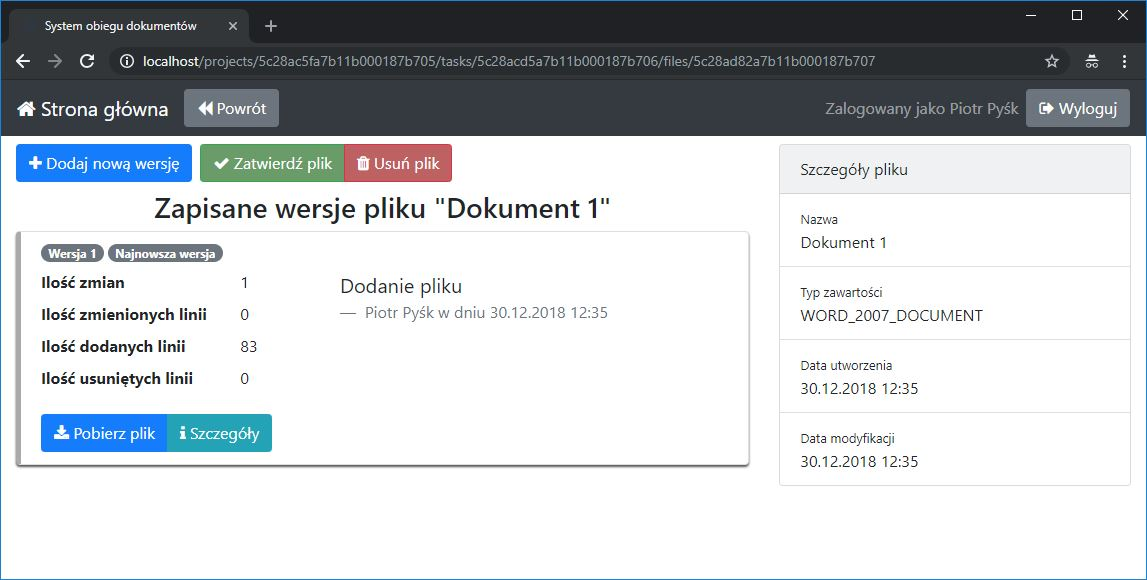
\includegraphics[width=0.8\textwidth]{figures/plik.jpg}
\caption{Widok szczegółowych informacji o pliku}
\label{fig:sysFunFile}
\end{figure}

\section{Architektura systemu i zakres zmian}

System został zaprojektowany i zaimplementowany zgodnie z architekturą wielowarstwową jako aplikacja internetowa.
Składa się z dwóch aplikacji: klienta przeglądarkowego i serwera aplikacyjnego.
Można wyróżnić w nim następujące warstwy:
\begin{itemize}
    \item \textbf{warstwa dostępu do danych} -- nadaje poziom abstrakcji ukrywając technologię stojącą za przechowywaniem danych systemu.
    Na jej poziomie następują bezpośrednie połączenia z~konkretną bazą danych i~komunikacją z~nią.
    Dzięki niej wymiana bazy danych sprowadziła się do zmian we właśnie tej warstwie.
    \item \textbf{warstwa logiki biznesowej} -- odpowiedzialna za główną logikę aplikacji, koordynuje jej pracę. 
    Ponadto jest odpowiedzialna za przetwarzanie i przekazywanie danych między warstwą dostępu do danych, a warstwą kontrolerów.
    Zmiany w tej warstwie ograniczyły się do sposobu użycia komponentów służących do dostępu do danych.
    \item \textbf{warstwa kontrolerów} -- najbardziej zewnętrzna warstwa w serwerze aplikacyjnym, wystawia sieciowy interfejs programowania aplikacji (ang.~\textit{WebAPI}) dla klienta przeglądarkowego.
    Jest odpowiedzialna za przyjmowanie i odpowiadanie żądania od niego poprzez wywoływanie odpowiednich procedur warstwy logiki biznesowej.
    Wymiana bazy danych nie powodowała jakichkolwiek zmian w tej warstwie systemu.
    Jest ona całkowicie niezależna od zastosowanej bazy i modelu danych.
    \item \textbf{warstwa prezentacji} -- klient przeglądarkowy, stanowi główny interfejs dla użytkownika systemu.
    Komunikuje się z warstwą kontrolerów i podobnie jak ona nie uległ jakimkolwiek modyfikacjom podczas zmiany bazy danych. 
\end{itemize}

\section{Stos technologiczny}

\subsection*{Projekty platformy Spring}

Duży wpływ na końcową architekturę aplikacji miał szkielet aplikacyjnym Spring.
Obecnie Spring jest platformą open-source złożoną z wielu projektów, która dedykowana jest do tworzenia aplikacji w języku Java.
Jego głównym elementem jest kontener wstrzykiwania zależności (ang.~\textit{dependency injection container}).
Szkielet aplikacyjny Spring sam instancjonuje i zarządza zależnościami komponentów aplikacji.
Dzięki tym mechanizmom zostaje przeniesiona funkcja sterowania wykonywaniem programu do używanego frameworku (ang.~\textit{Inversion of Control}) -- Spring sam w odpowiednich momentach wywołuje kod stworzony w ramach implementacji aplikacji.
Posiada również bogate wsparcie dla aplikacji internetowych, dostępu do baz danych, integracji z~innymi systemami przez najpopularniejsze protokoły komunikacyjne oraz walidacji danych \cite{SpringReference}.

W aplikacji zostały wykorzystane następujące komponenty platformy Spring:
\begin{itemize}
    \item \textbf{Spring Framework} -- podstawowy moduł wiążący w jedną całość pozostałe elementy.
    \item \textbf{Spring Boot} -- jeden z najważniejszych modułów, zapewnia prostszy i szybszy sposób konfigurowania i uruchamiania aplikacji.
    \item \textbf{Spring WebMVC} -- moduł zawierający rozszerzenia niezbędne do stworzenia aplikacji internetowej.
    \item \textbf{Spring Security} -- szkielet aplikacyjny, który umożliwia twórcom aplikacji narzucanie ograniczeń dostępu w aplikacjach internetowych bazujących na stosie technologii Spring.
    Posiada wsparcie m. in. dla uwierzytelniania przez integrację z LDAP, autoryzacji tylko uwierzytelnionych żądań HTTP.
    \item \textbf{Spring Data} -- projekt zawierający wiele modułów dostarczających narzędzi dostępu do najpopularniejszych baz i źródeł danych. 
    Wszystkie te moduły mają wspólny cel, którym jest ukrycie mnogości i złożoności technologii przechowywania danych poprzez ujednolicenie i usystematyzowanie terminologii z nimi związanych do abstrakcyjnych, niezależnych od technologii pojęć.
    \item \textbf{Spring Test} -- zestaw narzędzi ułatwiających testowanie aplikacji wykorzystujących szkielet aplikacyjny Spring z wykorzystaniem wybranych bibliotek do testowania takich jak JUnit lub TestNG. 
\end{itemize}

\subsection*{Apache Tika}

Apache Tika jest biblioteką open-source wydaną przez Apache Software Foundation na licencji Apache License 2.0, dzięki czemu można używać jej zarówno w otwartym oprogramowaniu jaki i komercyjnym. 
Zaopatruje ona system w bogatą kolekcję parserów i detektorów dla znacznej liczby popularnych formatów plików.
Oprócz tego umożliwia odczyt wielu metadanych plików.
Dzięki detektorom nie trzeba znać odgórnie formatu parsowanego pliku co jest znaczącą zaletą tej biblioteki.
W omawianym w pracy systemie jest wykorzystywana do parsowania zapisywanych w aplikacji dokumentów.
Wydobyta w tej sposób zawartość jest później wykorzystywana do wyszukiwania pełnotekstowego wśród plików.

\subsection*{DiffUtils}

Biblioteka DiffUtils posłużyła do porównywania dwóch sparsowanych wersji plików.
W pierwszej kolejności odczytany tekst jest dzielony na wektory z liniami, z których następnie DiffUtils oblicza różnice, które są zapisywane do bazy danych.
Do wyznaczania różnic biblioteka ta domyślnie wykorzystuje implementację algorytmu stworzonego przez Eugene'a W. Myers'a.
Została ona napisana w całości w języku Java.
Podobnie jak Tika, narzędzie to jest udostępnione na licencji Apache 2.0.

\section{Model danych}

Omawiane wcześniej aspekty systemu do prowadzenia projektów były wspólne dla wszystkich trzech jego wersji, które zostały zaimplementowane.
Poniżej został opisany sposób w jaki zostały zaprojektowane i zaimplementowane warstwy dostępu do danych w poszczególnych wersjach.
Wykorzystanie modułów projektu Spring Data we wszystkich wersjach skróciło w znacznym stopniu czas pracy nad systemem.
W systemie można wyróżnić następujące encje i ich atrybuty, które zostały przełożone na odpowiednie struktury danych w danej technologii:
\begin{itemize}
    \item \textbf{Użytkownik} -- obiekt reprezentujący zarejestrowanego użytkownika aplikacji. 
    Składa się z pól:
    \begin{itemize}
        \item unikalny adres e-mail, które służy do m. in. logowania się,
        \item hasło, które służy do logowania się do aplikacji,
        \item wyświetlane w aplikacji imię i nazwisko użytkownika.
    \end{itemize}
    
    \item \textbf{Projekt} agreguje grupę zadań.
    Posiada nazwę, opis, datę utworzenia oraz przypisanego administratora.
    Może też posiadać 0 lub więcej zadań.
    
    \item \textbf{Zadanie} podobnie jak projekt posiada nazwę, opis, datę utworzenia i administratora.
    Zadanie posiada również przypisanych uczestników i pliki.
    
    \begin{samepage}
    \item \textbf{Plik} -- obiekt zawierający informację o przypisanym do zadania pliku i jego wersjach.
    Posiada następujące atrybuty:
    \begin{itemize}
        \item nazwa, która w kontekście zadania jest unikalna,
        \item opis,
        \item datę utworzenia pliku w systemie,
        \item flagę czy plik został oznaczony do zatwierdzenia,
        \item flagę informującą czy plik został zatwierdzony przed administratora zadania,
        \item wykryty format pliku.
    \end{itemize}
    \end{samepage}
    
    \item \textbf{Wersja} pliku niesie ze sobą informacje o zmianach dokonanych w pliku.
    Nie może istnieć bez pliku, do którego jest przypisana.
    Ma następujące pola:
    \begin{itemize}
        \item data zapisu,
        \item numer wersji, który jest wykorzystywany do identyfikowania jej wśród innych wersji tego samego pliku,
        \item wiadomość kontrolna autora modyfikacji informująca o dokonanych zmianach,
        \item suma kontrolna służąca do weryfikacji poprawności odczytu pliku i do szybkiego porównania czy nowa wersja jest rzeczywiście inna od poprzednich,
        \item autor, który zapisał wersję,
        \item lista zmian względem poprzedniej wersji,
        \item właściwy plik, który został przesłany w~postaci binarnej -- może zostać pobrany z~systemu przez innych uczestników zadania,
        \item sparsowana zawartość pliku w postaci tekstowej, która podlega analizie i indeksowaniu w celu możliwości przeszukiwania pełnotekstowego pliku.
    \end{itemize}
    
    \item \textbf{Zmiana} reprezentuje informacje o pojedynczej modyfikacji dokonanej w pliku.
    Zawiera następujące dane:
    \begin{itemize}
        \item początkowy wiersz z poprzedniej wersji pliku, który uległ zmianie,
        \item ilość wierszy, która uległa zmianie w poprzedniej wersji,
        \item początkowy wiersz w nowej wersji pliku, który reprezentuje zmianę,
        \item ilość wierszy, która została zmieniona w nowej wersji pliku,
        \item typ dokonanej zmiany.
    \end{itemize}
\end{itemize}

Rysunek \ref{fig:domainObjects} obrazuje wszystkie wymienione encje na diagramie UML.

\begin{figure}[!ht]
\centering
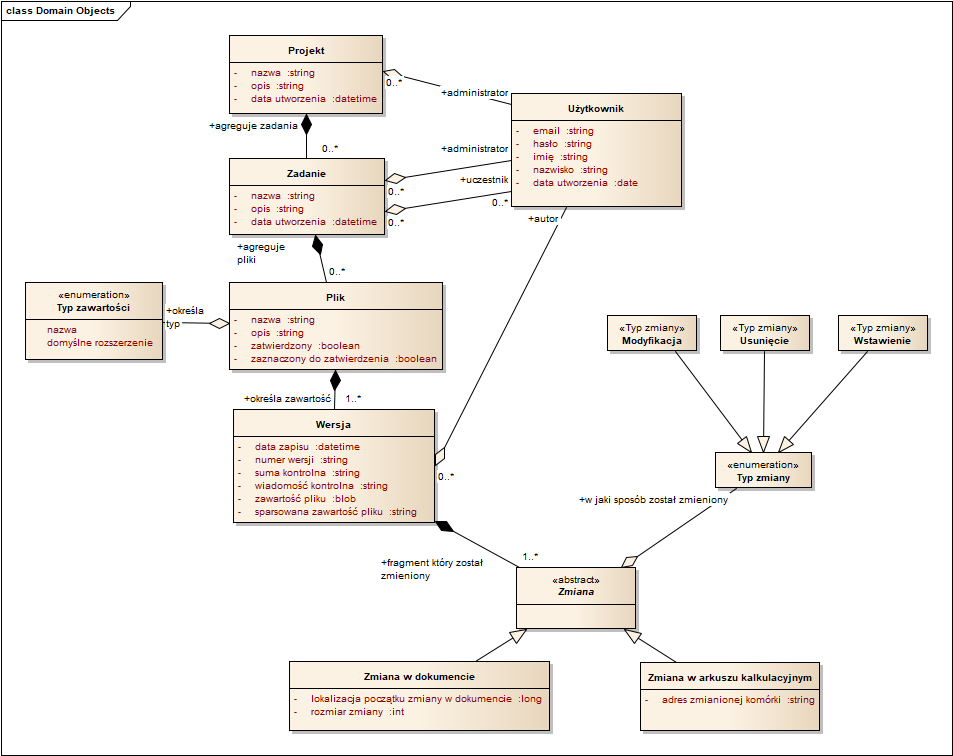
\includegraphics[width=\textwidth]{figures/domain_objects.png}
\caption{Model domenowy w opisywanym systemie}
\label{fig:domainObjects}
\end{figure}

\subsection*{Model danych przed dokonaniem zmian}

Przed dokonaniem zmian w warstwie dostępu do danych, system korzystał z relacyjnej bazy PostgreSQL~9.6.
Rysunek~\ref{fig:ModelPrzed} przedstawia diagram tabel schematu bazodanowego, z którego korzystał system przed zmianą bazy danych.
Większość tego modelu została przeniesiona do wersji systemu korzystającego z hybrydowego modelu danych i odpowiednio rozszerzona.
Opis tych tabel znajduje się w~sekcji~\ref{sec:hybridModel} na stronie~\pageref{sec:hybridModel}.

\begin{figure}[!ht]
\centering
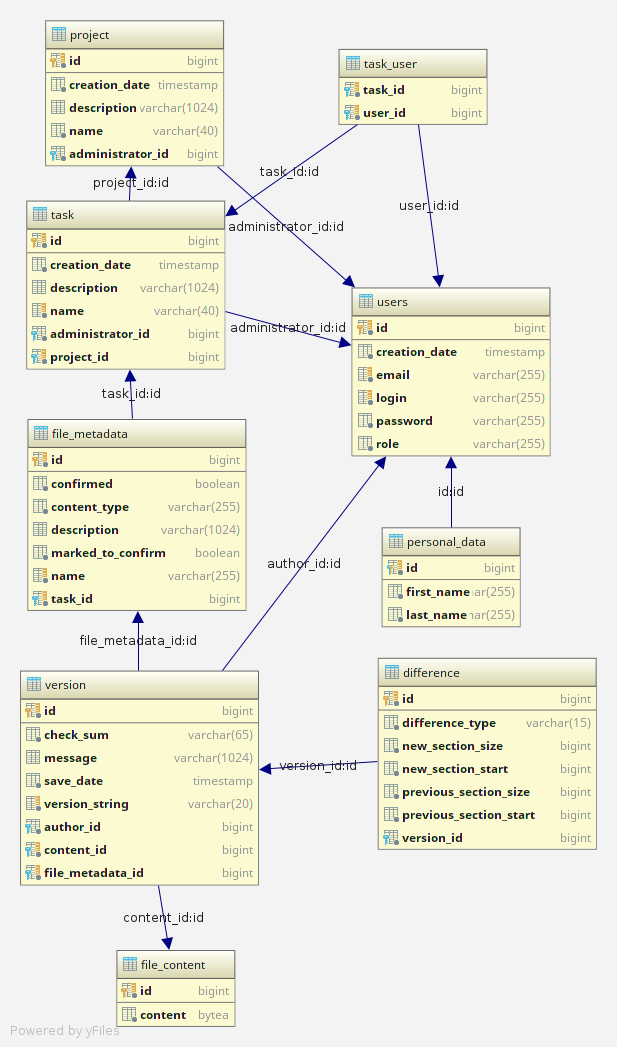
\includegraphics[width=0.85\textwidth]{figures/diagram_przed.png}
\caption{Diagram tabel modelu relacyjnego przed dokonaniem zmian}
\label{fig:ModelPrzed}
\end{figure}

\subsection{Model danych w Apache Cassandra + Elasticsearch} \label{sec:ModelDanychCassandra}

Pierwsza z wersji systemu korzysta z modyfikacji bazy danych Apache Cassandra w wersji~3.11 zintegrowanej z wtyczką Elasticsearch w~wersji~6.2.3 o~nazwie Elassandra.
Z powodu braku operacji złączenia w zapytaniach do Cassandry i potrzeby obsługi tej czynności po stronie aplikacji, część danych wymagała denormalizacji w celu skrócenia czasu potrzebnego na ich odczyt.
Dodatkowej konfiguracji wymagało mapowanie indeksu wtyczki Elasticsearch na wybraną tabelę.

\subsubsection{Niestandardowe struktury danych} \label{sec:cassadnraUDFs}

Na potrzeby aplikacji powstały niestandardowe typy danych, które zostały użyte w definicjach grup kolumn.
Rysunek~\ref{fig:CassandraUtd} przedstawia diagram z definicjami tych struktur.
Wśród nich możemy wyróżnić następujące typy:
\begin{itemize}
    \item \textbf{difference} -- struktura reprezentująca pojedynczą zmianę w dokumencie.
    \item \textbf{user\_summary} -- typ przechowujący krótkie podsumowanie informacji o użytkowniku.
    \item \textbf{file\_summary} -- struktura przechowująca krótkie podsumowanie informacji o pliku.
    \item \textbf{version\_summary} -- niestandardowy typ przechowujący krótkie podsumowanie informacji o wersji pliku.
\end{itemize}

\begin{figure}[!ht]
\centering
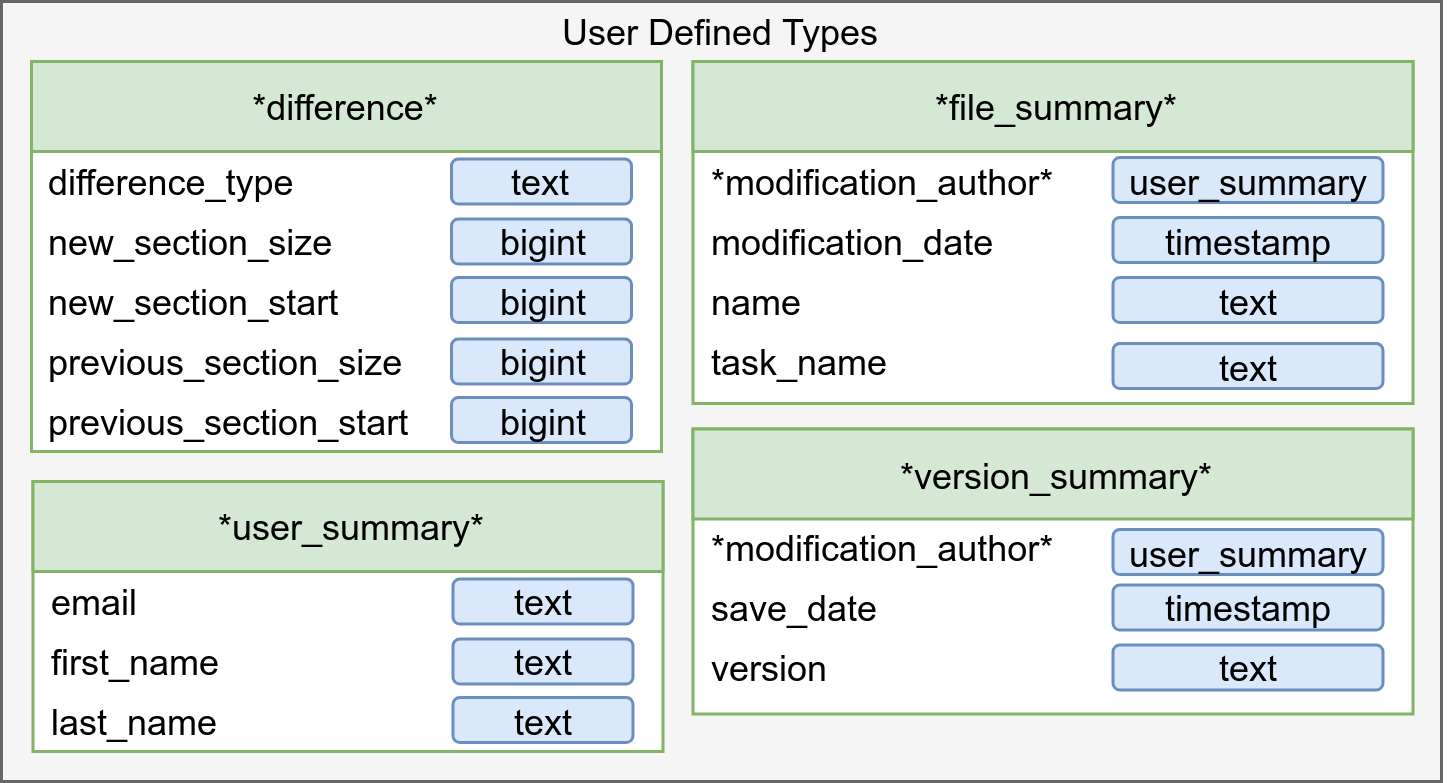
\includegraphics[width=0.9\textwidth]{figures/cassandra_udt.png}
\caption{Niestandardowe typy danych używanych przez system w~bazie Apache Cassandra}
\label{fig:CassandraUtd}
\end{figure}

\subsubsection{Grupy kolumn (nazywane w Cassandrze również tabelami)}

Rysunek~\ref{fig:CassandraTables} przedstawia diagram grup kolumn w~przestrzeni kluczy wykorzystywanej przez system.
W~przedstawionym modelu danych możemy wyróżnić następujące tabele:
\begin{itemize}
\begin{samepage}
    \item \textbf{user} -- tabela przechowująca dane o użytkownikach korzystających z systemu.
\end{samepage}

    \item \textbf{project} -- tabela przechowująca informacje o projektach.

    \item \textbf{user\_project} -- specjalna tabela przechowująca relację uczestnik projektu -- projekt. 
    Powstała w celu szybkiej weryfikacji czy dany użytkownik jest uczestnikiem projektu.
    Oprócz identyfikatorów użytkownika i projektu tabela zawiera informacje podsumowujące projekt. 
    Dane te są wyświetlane na liście projektów widocznej tuż po zalogowaniu do systemu.
    Powstała redundancja jest jednak rekompensowana szybkością operacji odczytu danych.

    \item \textbf{task} -- tabela przechowująca dane o zadaniach w systemie.
    Klucz główny jest złożony z kolumn \textit{project\_id} i \textit{task\_id}. 
    Kolumna \textit{project\_id} jest kluczem partycjonującym co zapewnia, że dane o zadaniach z jednego projektu będą przetrzymywane w jednym węźle.
    Kluczem sortującym dane w partycji jest kolumna \textit{task\_id}.

    \item \textbf{file\_metadata} -- tabela przechowująca dane o plikach zapisanych w systemie.
    Kluczem partycjonującym jest kolumna \textit{task\_id}, przez co informacje o plikach z jednego zadania są przechowywane na jednym węźle klastra.
    Dane w pojedynczej partycji są posortowane rosnąco według wartości w kolumnie \textit{file\_id}.

    \item \textbf{version} -- w tej tabeli przechowywane są dane o pojedynczej wersji pliku, wliczając w~to informacje o autorze modyfikacji, listę różnic względem poprzedniej wersji i zawartość pliku.
    Kluczem partycjonującym jest kolumna \textit{file\_id}, a dane są posortowane w odwrotnym porządku chronologicznym według kolumny \textit{save\_date}, przez co wyszukanie najnowszej wersji pliku, lub wybór wersji z danego przedziału czasowego jest bardzo szybki.
\end{itemize}

\begin{figure}[!ht]
\centering
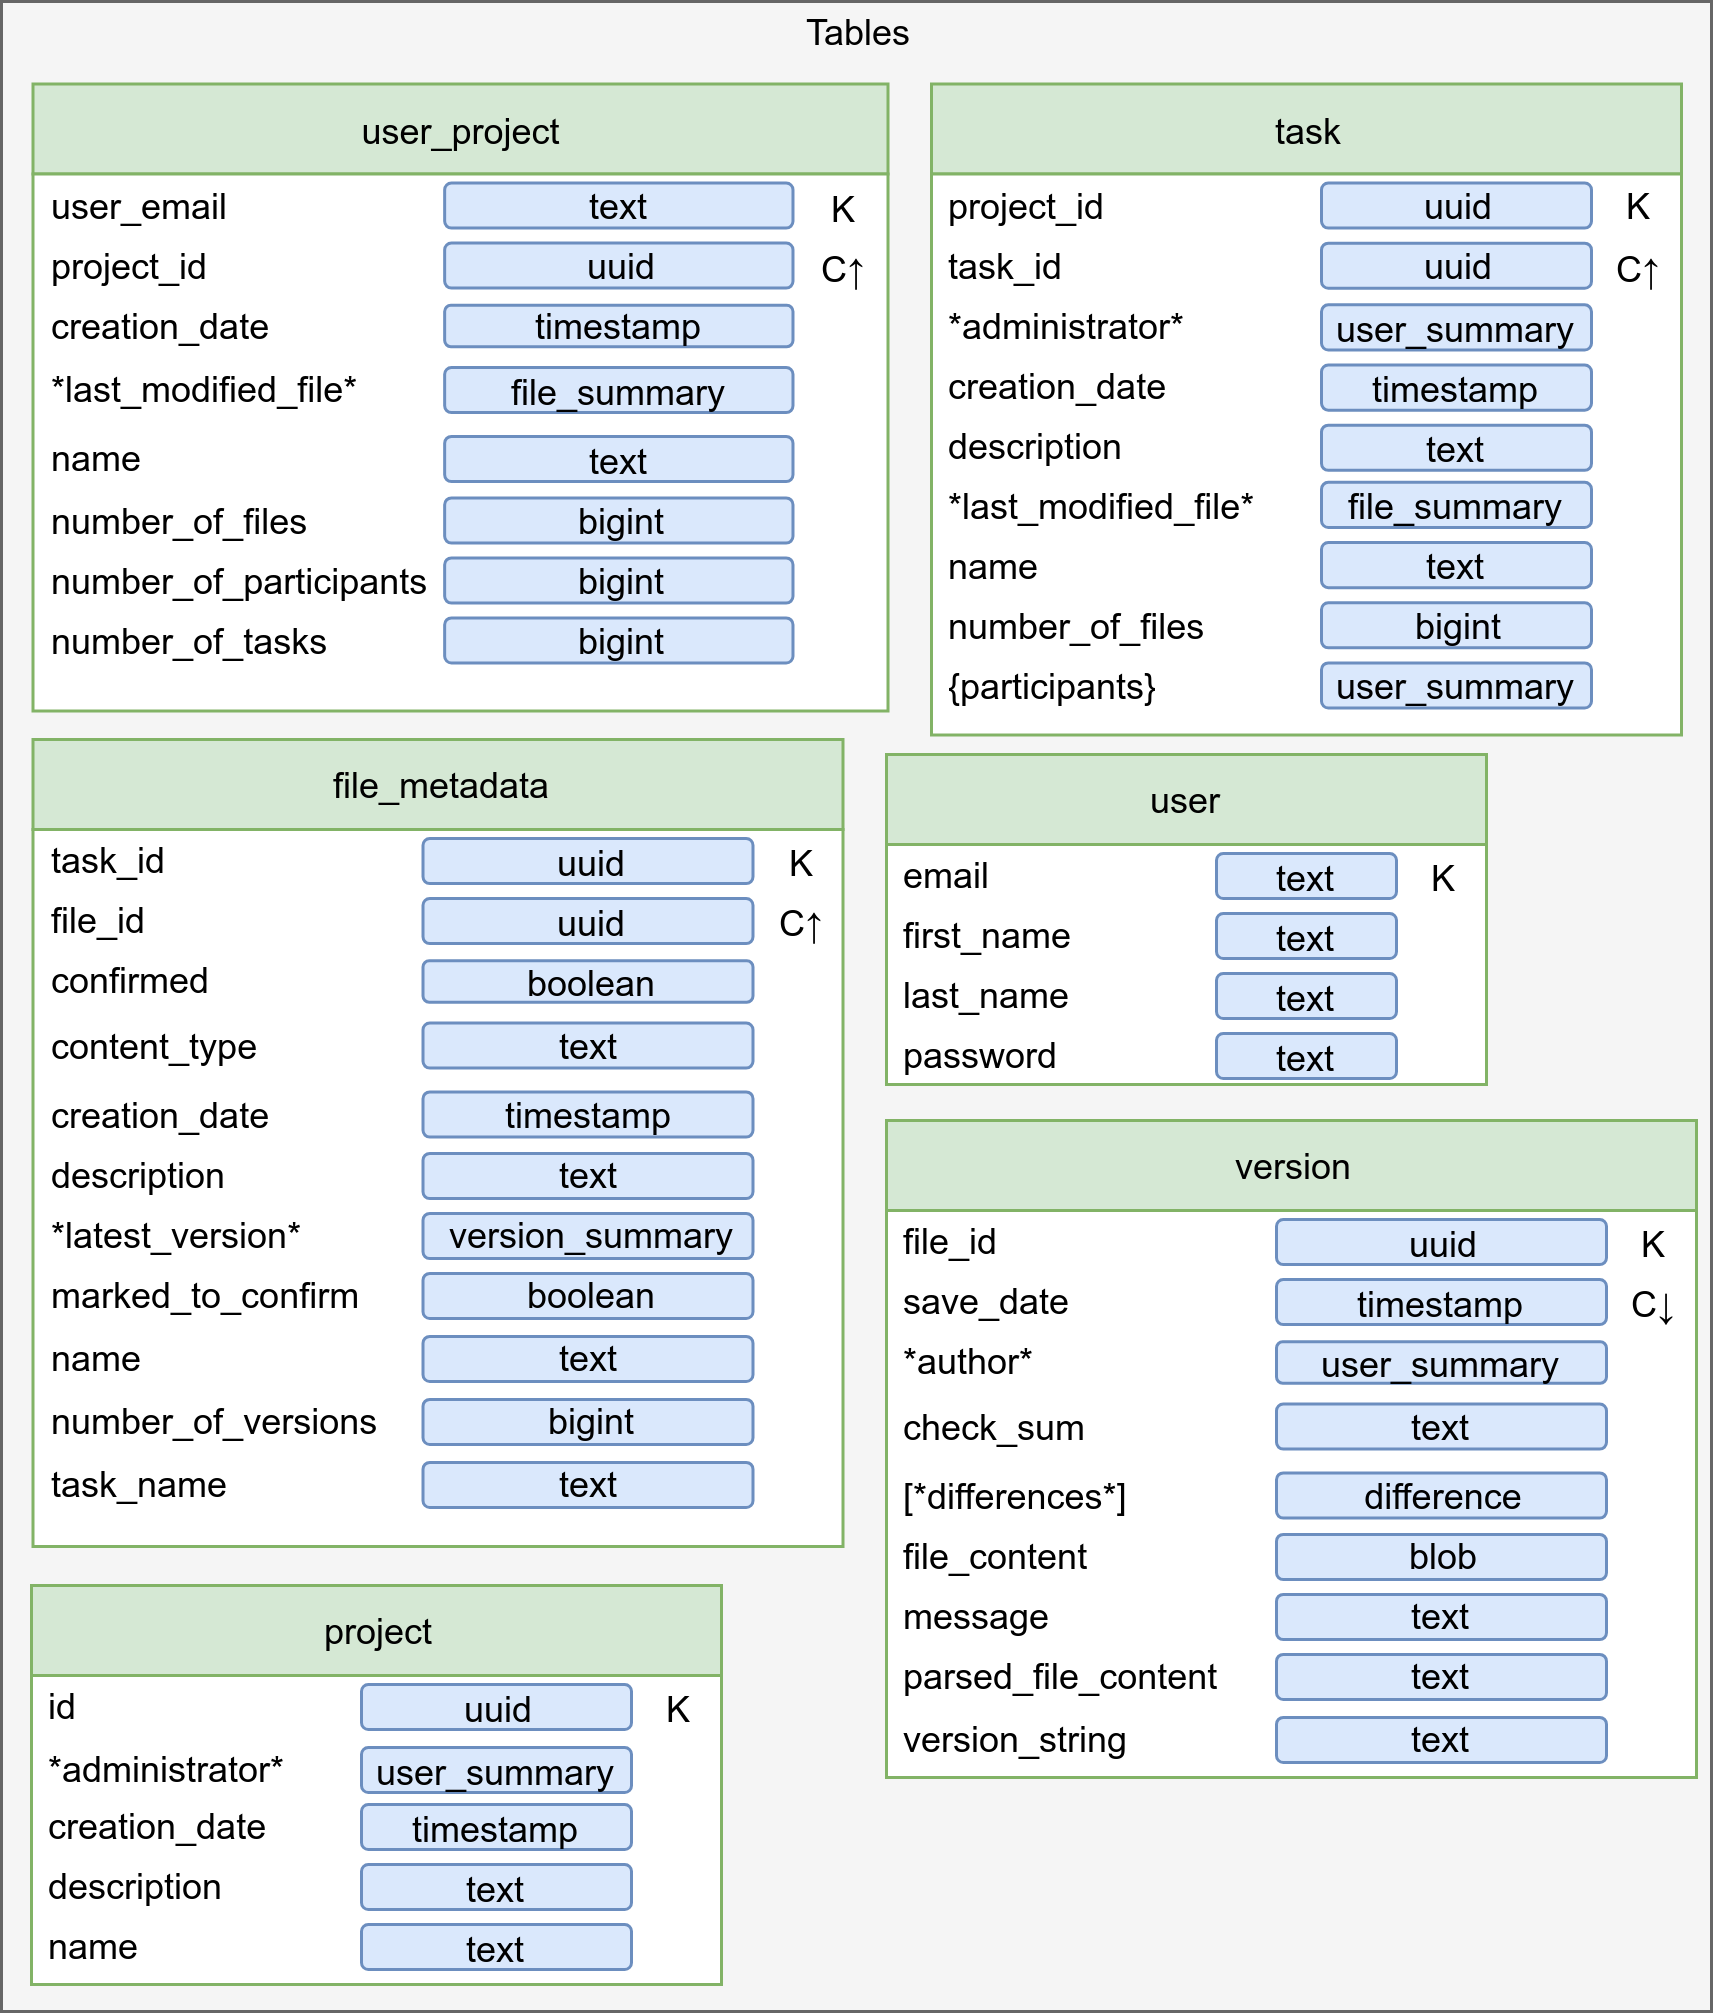
\includegraphics[width=0.9\textwidth]{figures/cassandra_tables.png}
\caption{Grupy kolumn używane przez opisywany system w~bazie Apache Cassandra}
\label{fig:CassandraTables}
\end{figure}

\subsubsection{Konfiguracja indeksowania tekstowego} \label{sec:cassandraTextIndexConfig}

W celu wyszukiwania pełnotekstowego zawartości plików tylko tabela \textit{version} podlegała indeksowaniu przez wtyczkę Elasticsearch,
a dokładnie jej kolumny:
\begin{itemize}
\begin{samepage}
    \item \textit{file\_id} -- identyfikator pliku,
\end{samepage}
    \item \textit{save\_date} -- data zapisu wersji,
    \item \textit{version\_string} -- wprowadzony przez autora numer wersji,
    \item \textit{message} -- wiadomość kontrolna,
    \item \textit{parsed\_file\_content} -- sparsowana zawartość pliku.
\end{itemize}

\subsection{Model danych w MongoDB}

Druga wersja systemu korzysta z bazy danych MongoDB w wersji 4.0.
Wszystkie powiązania do dokumentów, które są w innych kolekcjach zostały zaimplementowane z pomocą odwołania typu \textit{DBRef}, które zostały dokładniej opisane w sekcji \ref{sec:MongoModelDanych} na stronie \pageref{sec:MongoModelDanych}.
Dzięki temu dołączona do aplikacji biblioteka \textit{Spring Data for MongoDB} pobiera powiązane dokumenty, gdy zajdzie potrzeba. 
Każda, niżej wymieniona, kolekcja przechowuje zserializowane obiekty odpowiadającej jej klasy w aplikacji.
Rysunek~\ref{fig:MongoSchema} przedstawia diagram kolekcji w~bazie danych utworzonej przez system.
Model danych aplikacji obejmuje następujące kolekcje:
\begin{itemize}
    \item \textbf{user} -- kolekcja przechowująca informacje o zarejestrowanych użytkownikach.

    \item \textbf{project} -- kolekcja przechowująca dokumenty z informacjami o projektach.
    W celach wydajnościowych mogą one zawierać również powiązanie z ostatnio modyfikowanym plikiem oraz informacje o liczbie plików, zadań i uczestników w projekcie.
    
    \item \textbf{task} -- kolekcja przechowująca dokumenty z informacjami o zadaniach.
    Zawierają one pole z odwołaniem do projektów, do których są przypisane, oraz pole z odwołaniem do ostatnio modyfikowanego pliku.
    Relacja \textit{zadanie -- uczestnicy zadania} została zrealizowana za pomocą listy osadzonych dokumentów.
    
    \item \textbf{fileMetadata} -- kolekcja przechowująca dokumenty z metadanymi plików.
    Oprócz pól zdefiniowanych w encji pliku dokumenty posiadają odwołania do zadań, do których są przypisane.
    Dodatkowo posiadają również pole z referencją do najnowszej wersji pliku.
    
    \item \textbf{version} -- kolekcja przechowująca dokumenty z informacjami o wersjach plików.
    Posiada dodatkowy indeks na polu przechowującym datę zapisu wersji w celu szybszego odczytu najnowszej wersji pliku.
    Pola ze sparsowaną zawartością pliku i wiadomością kontrolną autora podlegają indeksowaniu pełnotekstowemu.
\end{itemize}

\begin{figure}[!ht]
\centering
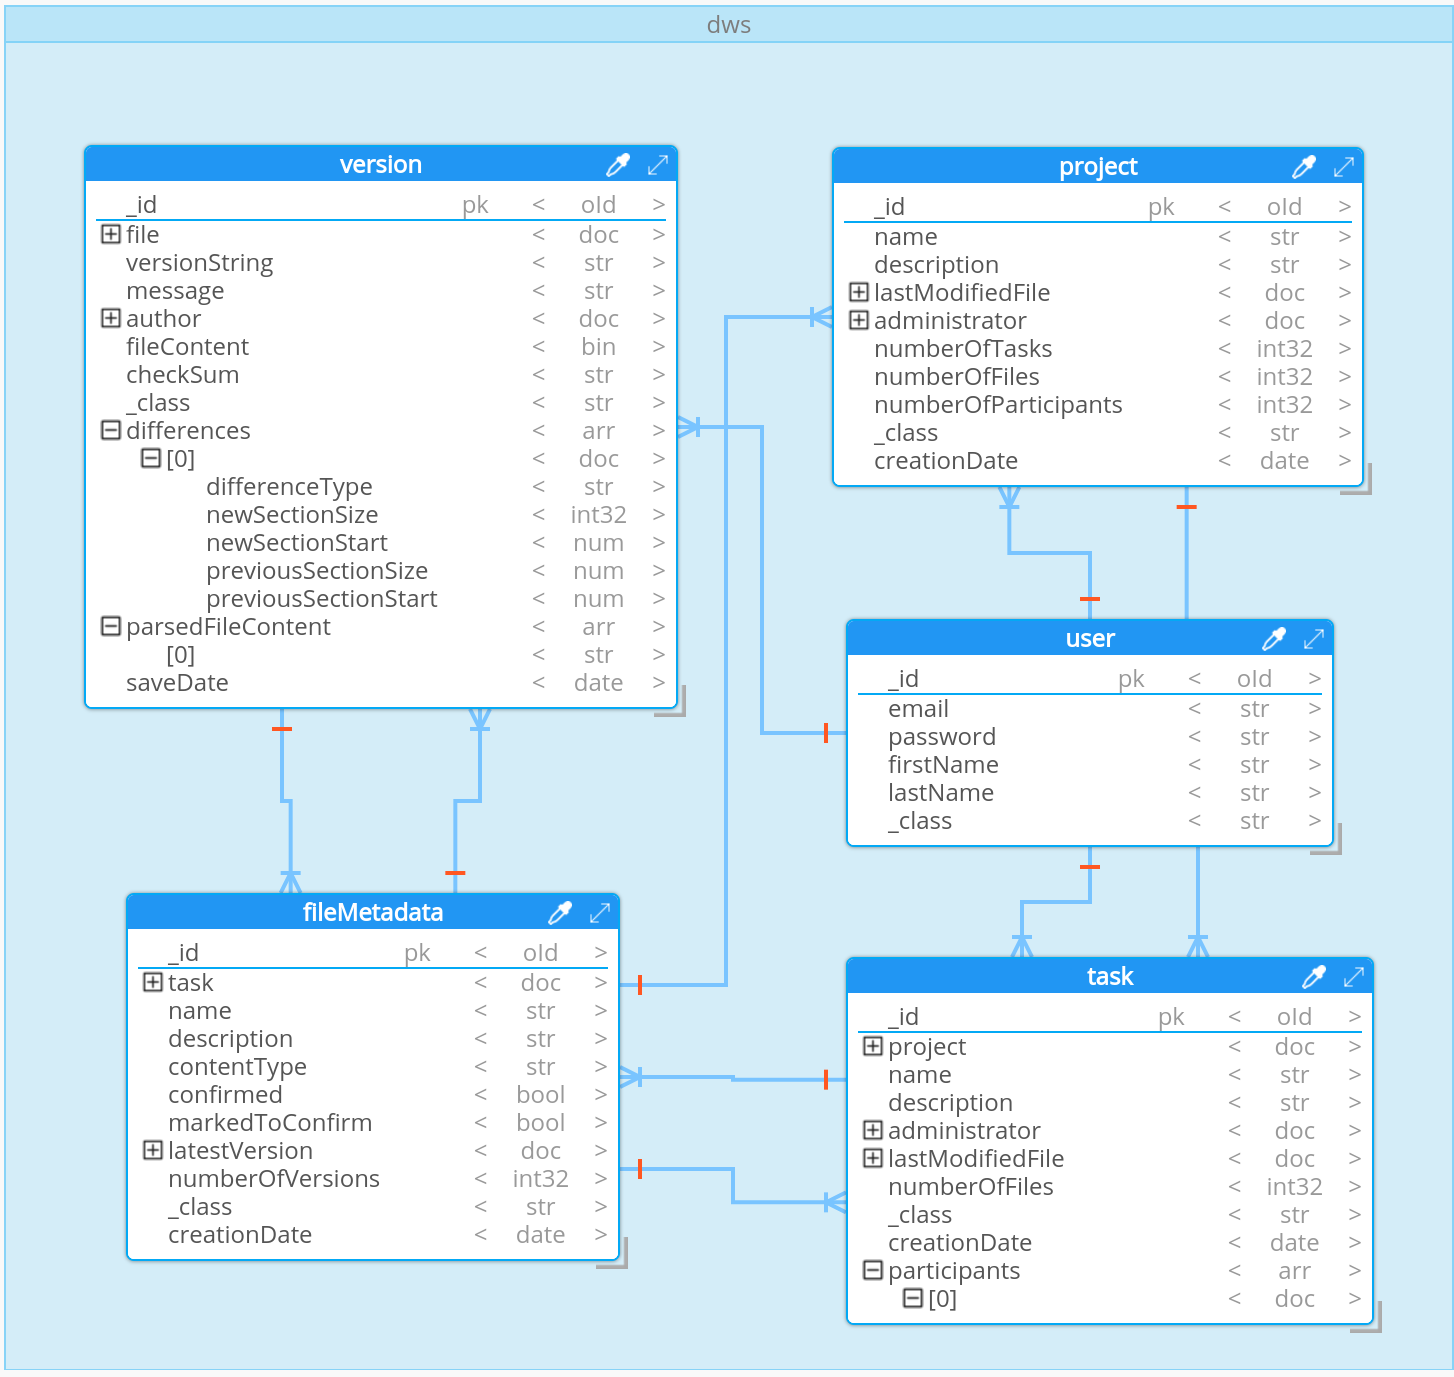
\includegraphics[width=0.95\textwidth]{figures/mongo_model.png}
\caption{Kolekcje i~związki między nimi w~bazie MongoDB wykorzystywanej przez opisywany system}
\label{fig:MongoSchema}
\end{figure}

\subsection{Model hybrydowy} \label{sec:hybridModel}

Trzecia wersja systemu bazuje na modelu hybrydowym -- dane \enquote{relacyjne} są przechowywane w~bazie PostgreSQL~10, a~krytyczne dla działania i~wydajności systemu dane są przechowywane w~bazie Apache Cassandra~3.11, wspomnianej w~sekcji~\ref{sec:ModelDanychCassandra}.

Przez dane krytyczne dla działania i wydajności systemu przyjęto informacje o wersjach plików, które mogą być najczęściej czytane, dodawane i modyfikowane przez użytkowników aplikacji.

\subsubsection{Część relacyjna}

Część relacyjna modelu hybrydowego działa w oparciu o bazę PostgreSQL 10, która jest jedną z najpopularniejszych i najbardziej dojrzałych darmowych rozwiązań wśród baz relacyjnych~\cite{DBEnginesRankingRDBMS}.
Ta część modelu powstała w oparciu o model domeny.
Na podstawie klas i ich atrybutów zostały zaprojektowane tabele.
Diagram przedstawiający ten fragment modelu znajduje się na Rysunku~\ref{fig:postgreModelDiag}.

\begin{figure}[!ht]
\centering
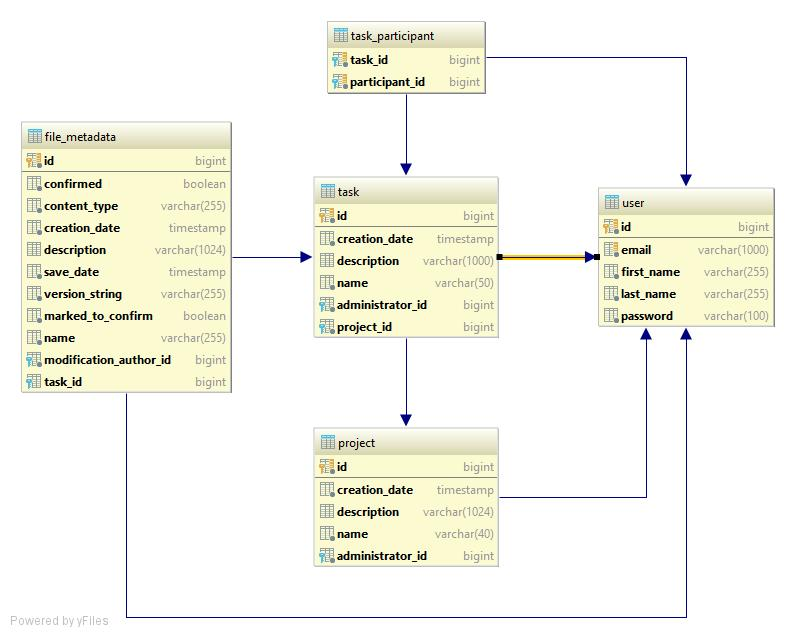
\includegraphics[width=0.8\textwidth]{figures/diagram.jpg}
\caption{Część relacyjna modelu hybrydowego}
\label{fig:postgreModelDiag}
\end{figure}

W tej części modelu możemy wyróżnić następujące tabele:
\begin{itemize}
\begin{samepage}
    \item \textbf{Tabela użytkowników -- user} \\ 
    Posiada dwa indeksy w celu przyspieszenia wyszukiwania użytkowników -- jeden na kluczu głównym, a drugi na kolumnie \textit{email}.
\end{samepage}
    
    \item \textbf{Tabela projektów -- project} \\
    Zawiera klucz obcy odnoszący się do rekordu w tabeli \textit{user}. 
    Identyfikuje on administratora projektu.
    
    \item \textbf{Tabela zadań -- task} \\
    Zawiera klucz obcy odnoszący się do administratora zadania, oraz klucz do projektu, do którego zadanie jest przypisane.
    
    \item \textbf{Tabela asocjacyjna -- task\_participant} \\
    Tworzy relację wiele do wielu pomiędzy uczestnikami zadania i zadaniami, w których użytkownik bierze udział. 
    Posiada dwa kolumny, które są jednocześnie kluczami obcymi do tabel zadań i użytkowników. 
    Wpisy nie mogą zawierać pustych wartości, oraz nie mogą się duplikować przez nałożenie unikalności na każdy wiersz.
    
    \item \textbf{Tabela metadanych plików -- file\_metadata} \\
    Przechowuje klucz obcy do zadania, do którego jest przypisany plik.
    Posiada nałożone ograniczenie na unikalność par wartości \textit{name} i \textit{task\_id}, aby nazwy plików nie powtarzały się w tym samym zadaniu.
\end{itemize}

\subsubsection{Część nierelacyjna}

Część nierelacyjna oparta na Cassandrze 3.11 z wtyczką Elasticsearch 6.3.2 składa się z~jednej tabeli o nazwie \textit{version}.
Używa ona niestandardowych struktur danych, których definicje zostały opisane w sekcji \ref{sec:cassadnraUDFs} na stronie \pageref{sec:cassadnraUDFs}.
Różnica między nią, a~tabelą \textit{version} z modelu bazującego w~całości na Cassandrze, polega na tym, że kolumna \textit{file\_id} jest typu \textit{bigint}.
Ma to na celu przechowywanie identyfikatorów plików, które w~bazie PostgreSQL są liczbami całkowitymi.
Rysunek~\ref{fig:hybridCassandraPart} przedstawia diagram z~definicją tej tabeli.
Pominięto na nim definicje niestandardowych struktur danych, które są identyczne co ich odpowiedniki w~modelu danych bazy Cassandra.

\begin{figure}[!ht]
\centering
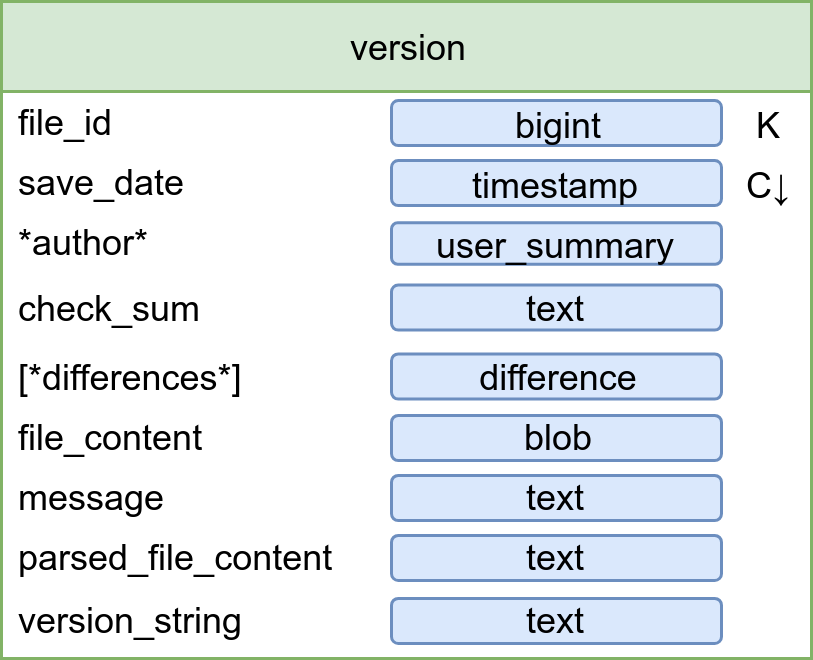
\includegraphics[width=0.6\textwidth]{figures/hybrid_cassandra_model.png}
\caption{Część nierelacyjna hybrydowego modelu danych}
\label{fig:hybridCassandraPart}
\end{figure}

Konfiguracja indeksowania pełnotekstowego przez wtyczkę Elasticsearch pozostaje również identyczna co modelu bazującym tylko na samej Cassandrze. 
Została ona opisana na stronie~\pageref{sec:cassandraTextIndexConfig} niniejszej pracy.
